\newif\ifjapanese

\japanesetrue

\documentclass[11pt]{jreport}
\renewcommand{\bibname}{参考文献}
\newcommand{\acknowledgmentname}{謝辞}

\usepackage{ascmac}
\usepackage{graphicx}
\usepackage{multirow}
\usepackage{ylab_thesis}
\usepackage{listings}

% 自作
\newcommand{\sun}[0]{_{\odot}}


\bindermode

\jclass{卒業論文}
\jtitle{恒星の進化と爆発過程の\\数値シュミレーション}
\juniv{東京理科大学}
\jfaculty{理工学部物理学科}
\jauthor{高橋 倖平}
\jadvisor{鈴木 英之}{教授}
\jhyear{31}
\jsyear{2019}
\jkeyword	{MESA,重力崩壊型超新星爆発,ニュートリノ加熱}

\begin{document}

\jmaketitle

% アブストラクト
\begin{jabstract}

太陽の何十倍もの質量のある星は,一生の終わりに,超新星により中性子性を残したり,ブラックホールを形成したりする.しかし,現在,どんな構造の星がそれらの過程のどれを経るのかは明確に分かっていない.そこで,実際に星の最後がどうなるのかを調べるため,爆発時の過程をコードを作成し計算を行った.計算は前半と後半で分かれており,前半部分は爆発直前の親星の構成を計算し,後半部分は重力崩壊を始めてから衝撃波が星の表面まで到達するまでの過程を追い,最終的に爆発時の爆発のエネルギーを求めた.手法としては,MESA\cite{mesa}で前半部分を,m\"{u}llerの論文\cite{muller}を元にした自作のコードで後半部分をという手法で行った.

\end{jabstract}


\tableofcontents
\listoffigures

\pagenumbering{arabic}

\chapter{序論}
\label{chap:introduction}

本研究の背景や本論文の構成を書く.


\section{背景}

太陽の何十倍もの質量のある星は,一生の終わりに,超新星により中性子性を残したり,ブラックホールを形成したりする.しかし,現在,どんな構造の星がそれらの過程のどれを経るのかは明確に分かっていない.今回は個々の星について考え,重力崩壊型超新星爆発を起こすケースにおいて超新星爆発後にどのくらいのエネギーを持っていて,さらに放出される元素が何であるかを調べる.そして,その結果を多くの星が集合をなす銀河系に応用できるようにしていく.


\section{本文書の構成}

第\ref{chap:introduction}章では本卒論の概要みたいなのを書いた.第\ref{chap:supernova}章では、主に今回の計算で必要な基本的な現状についてであり,重力崩壊後,爆発を起こすまでの過程についてを説明する.第\ref{chap:mesa_method}章と第\ref{chap:muller_calc}章では,主に計算に用いたコードについてであり,第\ref{chap:mesa_method}章ではMESAを用いた計算の手法について,第\ref{chap:muller_calc}章では重力崩壊後から爆発に到るまでの数値計算の方法についてを説明する.

\chapter{重力崩壊型超新星爆発}
\label{chap:supernova}

この章では、重力崩壊後から爆発を起こすまでの様子を3つのフェーズに分けて説明していく.最初のフェーズはコア反跳によって生成された衝撃波が停滞している状態で,これを「爆発前段階」と呼ぶ.次の段階は衝撃の停滞がニュートリノ加熱によって解除され徐々に広がっている段階で,これを「爆発段階(Phase1)」と呼ぶ.最後のフェーズは衝撃波のエネルギーが落ちてくる物質を外に全て跳ね返すほど大きくなる状態で,これを「爆発段階(Phase2)」と呼ぶ.この3つのフェーズについて以下で見ていく.

\section{爆発前段階}

ここでは停滞した衝撃波が復活するかどうかを考える.衝撃波の外側から中心に向かって降着してくる物質はゲイン領域を通過する時にニュートリノからエネルギーを受け取るが,その受け取ったエネルギーが重力的な結合エネルギーを上回ることができると衝撃波が復活するようになる.ここでは,ゲイン領域内の降着物質に注目する.
\subsection{降着物質の降着率}

降着物質は重力崩壊直前星における中心から位置$r$にある質量シェル(密度$\rho$)が落ちてきたものである.この時,物質は自由落下で落ちてきていると仮定して,落ちてくるまでのタイムスケールは自由落下のタイムスケールの定数倍となる.したがって,ある質量シェルが中心まで落ちてくる時間は
$$
t=\sqrt{\frac{\pi}{4G\bar{\rho}}}\eqno{(2.1)}
$$
と表せる.ここで,$\bar{\rho}$は重力崩壊前の質量シェルにおける半径$r$の位置での平均密度である.以下の式で表される.
$$
\bar{\rho}=\frac{M}{\frac{4}{3}\pi r^3}\eqno{(2.2)}
$$
結果として,生じる質量降着率は,次のように表される.
$$
\dot{M}=\frac{2M}{t}\frac{\rho}{\bar{\rho}-\rho}\eqno{(2.3)}
$$

\subsection{ゲイン半径}

ゲイン半径$r_g$では,降着物質がその重力的なポテンシャルエネルギーの約半分を失い,ゲイン半径での光度$\frac{GM\dot{M}}{2r_g}$として失う.このことから,
$$
M^4r_g^2\propto\frac{GM\dot{M}}{2r_g}\eqno{(2.4)}
$$
つまり,
$$
r_g\propto\frac{\dot{M}^{1/3}}{M}\eqno{(2.5)}
$$
と表される.しかし,これは明らかに$\dot{M}$が小さい場合におかしな値になるので,下限値として中性子星の半径$r_0$を補完する.すると,ゲイン半径は以下のように表せる.
$$
r_g=\sqrt[3]{r_1^3\left(\frac{\dot{M}}{M\sun}\right)\left(\frac{M}{M\sun}\right)^{-3}+r_0^3}\eqno{(2.6)}
$$
計算では,$r_0=12\rm{km}$,$r_1=120\rm{km}$を用いる.
\subsection{衝撃波半径}

ゲイン半径が決定すると,衝撃波半径を決定することができる.ゲイン半径では,単位質量あたりのニュートリノの加熱速度と冷却速度が釣り合っている.そのことを考えると,
$$
T^6_g\propto\frac{L_{\nu}E_{\nu}^2}{r_g^2}\eqno{(2.7)}
$$
ここで,$P_g\propto T_g^4$であるから,
$$
P^{3/2}_g\propto\frac{L_{\nu}E_{\nu}^2}{r_g^2}\eqno{(2.8)}
$$
となる.

ここで,衝撃波の前後での密度の比を$\beta=\frac{\rho_{pre}}{\rho_{sh}}$とする.そして,衝撃波直前の速度$v_{pre}$が自由落下時の速度になることから
$$
v_{pre}=\sqrt{\frac{2GM}{r_{sh}}}\eqno{(2.9)}
$$
となり,これを用いて衝撃波直前の密度が
$$
\rho_{pre}=\frac{\dot{M}}{4\pi r2v_{pre}}\eqno{(2.10)}
$$
として得られることから,衝撃波での圧力$P_{sh}$が次のように決まる.
$$
P_{sh}=\frac{\beta-1}{\beta}\rho_{pre}v_{pre}^2\eqno{(2.11)}
$$
この式と式(8)を合わせると,
$$
r_{sh}\propto\frac{(L_{\nu}E^2_{\nu})^{4/9}r_g^{16/9}}{\dot{M}^{2/3}M^{1/3}}\propto\frac{L_{\nu}^{4/9}M^{5/9}r_g^{16/9}}{\dot{M}^{2/3}}\eqno{(2.12)}
$$
となる.ここで多次元での衝撃波の復活で理論的に推定された値の標準値$\alpha_{turb}\sim1.18$を用いて
$$
r_{sh}=\alpha_{turb}\times0.55\rm{km}\times\left(\frac{L_{\nu}}{10^{52}\rm{erg s^{-1}}}\right)^{4/9}\times(\alpha^3)^{4/9}\times\left(\frac{M}{M\sun}\right)^{5/9}\times\left(\frac{r_g}{10\rm{km}}\right)^{16/9}\times\left(\frac{M}{M\sun}\right)^{-2/3}\eqno{(2.13)}
$$
\subsection{ニュートリノ光度}

衝撃半径を計算する時にも必要なニュートリノ光度$L_{\nu}$について説明する.衝撃波半径に向かってニュートリノが飛び出してくるのには2種類の起源がある.1つは降着物質の重力的な結合エネルギーが変換されニュートリノが出てくる事によるニュートリノ光度$L_{acc}$で,もう1つは中性子星が時間経過によって冷やされることで放出されるニュートリノ光度$L_{diff}$である.

まず,降着成分によるニュートリノ光度$L_{acc}$であるが,これは,パラメータ$\zeta$を用いて,
$$
L_{acc}=\zeta\frac{GM\dot{M}}{r_g}\eqno{(2.14)}
$$
と表される.計算では,パラメータ$\zeta=0.71$を用いた.

次に,中性子星によるニュートリノ光度$L_{diff}$であるが,これは中性子星の結合エネルギー$E_{bind}$と冷却時間$\tau_{cool}$から求めることができる.
$$
L_{diff}=0.3\times\frac{E_{bind}}{\tau_{cool}}e^{-t/\tau_{cool}}\eqno{(2.15)}
$$
ここで,中性子星の結合エネルギー$E_{bind}$と冷却時間$\tau_{cool}$については以下を用いる.
$$
E_bind=0.084\times\left(\frac{M}{M\sun}\right)^2M\sun c^2\eqno{(2.16)}
$$

$$
\tau_{cool}=\tau_{1.5}\times\left(\frac{M}{1.5M\sun}\right)^{5/3}\eqno{(2.17)}
$$

これらにより,ニュートリノ光度$L_{\nu}$は
$$
L_{\nu}=L_{acc}+L_{diff}\eqno{(2.18)}
$$
で求められる.ここまでで,ゲイン半径$r_g$と衝撃波半径$r_{sh}$を求めることができた.

\subsection{加熱条件}

衝撃波を通過した降着物質がゲイン半径で重力的束縛エネルギーを超えるだけのニュートリノ加熱を得ることができた時,衝撃波の停滞は終わり衝撃波は復活をする.降着物質がゲイン領域を通過する時間を$\tau_{adv}$,降着物質がニュートリノから重力的な結合エネルギーを超えるエネルギーを得るのにかかる時間を$\tau_{heat}$とすると,衝撃波が復活する条件は,
$$
\tau_{heat}<\tau_{adv}\eqno{(2.19)}
$$
となる.

降着物質がゲイン領域を通過する時間$\tau_{adv}$は第一原理シュミレーションにより係数が設定され,
$$
\tau_{adv}=\frac{\int^{r_{sh}}_{r_g}4\pi r^2\beta\rho_{pre}(r_{sh}/r)^3\rm{dr}}{\dot{M}}\sim18\rm{ms}\left(\frac{r_{sh}}{100\rm{km}}\right)^{3/2}\left(\frac{M}{M\sun}\right)^{-1/2}\ln{\frac{r_{sh}}{r_g}}\eqno{(2.20)}
$$
と表される.

降着物質がニュートリノから重力的な結合エネルギーを超えるエネルギーを得るのにかかる時間$\tau_{heat}$は,ニュートリノの平均加熱率$\dot{q}_{\nu}$と平均結合エネルギー$e_g$で表すとができる.
$$
\tau_{heat}=\frac{|e_g|}{\dot{q}_{\nu}}\eqno{(2.21)}
$$
ここで,ニュートリノの平均加熱率$\dot{q}_{\nu}$は,
$$
\dot{q}_{\nu}\propto\frac{L_{\nu}E_{\nu}^2}{r_g^2}\eqno{(2.22)}
$$
と表すことができる.平均結合エネルギー$e_g$については,球対称のベルヌーイの定理を用いることで推定できる.総エンタルピー$h$と運動エネルギー密度$\frac{v^2}{2}$と重力ポテンシャル$\Phi$が保存すると考えるので,
$$
h+\frac{v^2}{2}+\Phi=0\eqno{(2.23)}
$$
と書ける.これを降着物質に当てはめると,
$$
\left(\epsilon_{therm}+\epsilon_{diss}+\frac{P_{sh}}{\rho_{sh}}\right)+0-\frac{GM}{r_{sh}}\sim0\eqno{(2.24)}
$$
と表される.ここで,衝撃波直後の単位質量あたりのエネルギーを$\epsilon_{therm}$とし,そのうちの静止質量の寄与を$\epsilon_{diss}$としている.また,放射圧の影響が強いため,$P_{sh}/\rho_{sh}=\epsilon/3$とできる.これを解くと,
$$
\epsilon_{therm}=\frac{4}{3}\left(\frac{GM}{r_{sh}-\epsilon_{diss}}\right)\eqno{(2.25)}
$$
よって,静止質量の寄与が無い衝撃波通過後の結合エネルギー$|e_g|$は,
$$
|e_g|=|\epsilon_{therm}-\frac{GM}{r_{sh}}|=\frac{3}{4}\epsilon_{diss}+\frac{GM}{4max(r_{sh},r_g)}\eqno{(2.26)}
$$
と表される.ここで,重い原子核が落下中に完全に核子に分離されると想定すると$\epsilon_{diss}\sim8.8\rm{MeV}$とでき,計算でもこの値を用いた.

したがって,式(22)(23)より,加熱のタイムスケール$\tau_{heat}$は,
$$
\tau_{heat}=150\rm{ms}\times\left(\frac{|e_g|}{10^{19}\rm{erg g^{-1}}}\right)\times\left(\frac{r_g}{100\rm{km}}\right)^2\times\left(\frac{L_{\nu}}{10^{52}\rm{erg s^{-1}}}\right)^{-1}\times(\alpha^3)^{-1}\times\left(\frac{M}{M\sun}\right)^{-2}\eqno{(2.27)}
$$
となる.これで式(19)を評価することができる.式(19)を満たしたら次に説明する,爆発段階(Phase1)に進む.

\section{爆発段階(Phase1)}

この段階では,衝撃波が復活しているが衝撃波に達した降着物質が全て吹き飛ばされるわけではなく,まだ衝撃波を通過する降着物質が多いという状況を考えている.つまり,降着率$\dot{M}_{acc}$と外に出て行く質量率$\dot{M}_{out}$が以下の関係にあると考える.
$$
\dot{M}_{acc}\gg\dot{M}_{out}\eqno{(2.28)}
$$
これは衝撃波を通過した降着物質の速度$v_{post}$が脱出速度$v_{esc}$を超えていないためである.つまりこのフェーズの終わりの条件は,
$$
v_{post}>v_{esc}\eqno{(2.29)}
$$
となる時である.脱出速度$v_{esc}$は簡単に求まり,
$$
v_{esc}=\sqrt{\frac{2GM}{r}}\eqno{(2.30)}
$$
である.衝撃波を通過した降着物質の速度$v_{post}$は圧縮比$\beta_{expl}$を用いて,
$$
v_{post}=\frac{\beta_{expl}-1}{\beta_{expl}}v_{sh}\eqno{(2.31)}
$$
として表される.以下では,衝撃波の速度$v_{sh}$を求める.

\subsection{爆発のエネルギー}

衝撃波の速度$v_{sh}$は,衝撃波を通過してバラバラになった物質がニュートリの加熱によって外向きに進み,その降着物質が再結合した際に放出されるエネルギーに依存するものである.よって,そのエネルギーを爆発のエネルギー$E_{diag}$とし,先にこれを求めることにする.この爆発のエネルギー$E_{diag}$は累次的に足し合わせて行くことで最終的には重力崩壊型超新星爆発の爆発エネルギーとなる.

爆発のエネルギー$E_{diag}$は,
$$
\frac{\rm{d} E_{diag}}{\rm{d} M_{sh}}=\frac{(1-\alpha_{out})\epsilon_{rec}\eta_{acc}}{|e_g|}+\alpha_{out}(\epsilon_{bind}+\epsilon_{burn})\eqno{(2.32)}
$$
と表される.ここで,$1-\alpha_{out}$の部分が衝撃波を通過する割合を表しており,$\epsilon_{rec}$が再結合のエネルギーを表している.計算では再結合のエネルギー$\epsilon_{rec}=5\rm{MeV}$を使用する.また,ニュートリノ加熱の影響以外にも,結合エネルギー$\epsilon_{bind}$と核燃焼エネルギー$\epsilon_{burn}$についても考えたのが第2項目である.結合エネルギー$\epsilon_{bind}$については,計算の際にデータとして持ってきて計算を行う.

核燃焼エネルギー$\epsilon_{burn}$については,以下のフラッシングメソッドを用いて計算を行う.


\subsection{フラッシングメソッド}

この「フラッシングメソッド」では,ある一定の温度に達したら核燃焼が一瞬のうちに起こると仮定するもので,衝撃波の温度によって燃焼の段階が変わるというものである.衝撃波の温度については,降着物質の速度が衝撃波の速度より無視できるほど小さいと仮定すると,
$$
P_{sh}=\frac{aT^4_{sh}}{3}=\frac{\beta_{expl}-1}{\beta_{expl}}\rho v^2_{sh}\eqno{(2.33)}
$$
より,次のように求まる.
$$
T_{sh}=\sqrt[4]{\frac{3(\beta_{expl}-1)}{\beta_{expl}}\rho v^2_{sh}}\eqno{(2.34)}
$$
この衝撃波の温度$T_{sh}$によって以下のように組成が変化するとする.
\begin{enumerate}
  \item $2.5\times10^{9}\rm{K}\leq T_{sh}<3.5\times10^{9}$の場合,Oよりも軽い元素が$^{16}$Oまで燃焼する
  \item $3.5\times10^{9}\rm{K}\leq T_{sh}<5.0\times10^{9}$の場合,Siよりも軽い元素が$^{28}$Siまで燃焼する
  \item $5.0\times10^{9}\rm{K}\leq T_{sh}<T_{\alpha}$の場合,Niよりも軽い元素が$^{56}$Niまで燃焼する
\end{enumerate}
この$T_{\alpha}$とは$\alpha$粒子の質量関数が0.5になる時の密度に依存する温度を表し,次の式で与えられる.
$$
\log_{10}{\rho}=11.62+1.5\log_{10}{\left(\frac{T_{\alpha}}{10^9\rm{K}}\right)}-39.17\left(\frac{T_{\alpha}}{10^9\rm{K}}\right)^{-1}\eqno{(2.35)}
$$
計算上では,これをニュートン法をもちいて計算する.そして再帰的に以下の核燃焼エネルギー$\epsilon_{burn}$は,
$$
\epsilon_{burn}=\sum_i X_i\left(\frac{m_i}{A_i}-\frac{m_{end}}{A_{end}}\right)\frac{c^2}{mu}\eqno{(2.36)}
$$
と計算される.ここで,$X_i$は元素$i$の質量分立,$A_i$は元素$i$の質量数,添字$end$は燃焼後に最終的に変化する元素のことを表す.

\subsection{衝撃波速度}

フラッシングメソッドによって,核燃焼エネルギーが求まると爆発のエネルギーを計算でき,最終的に衝撃波の速度を求めることができる.
$$
v_{sh}=0.794\left(\frac{E_{diag}}{M-M_{ini}}\right)^{1/2}\left(\frac{M-M_{ini}}{\rho r^3}\right)^{0.19}\eqno{(2.37)}
$$
ここで出てくる$M_{ini}$は「爆発前段階」における移行直前の質量のことである.

以上により,式(29)の条件を計算できるようになり,次のフェーズに移行するかどうかを判断することができる.


\section{爆発段階(Phase2)}

この段階では,衝撃波に到達した降着物質が全て外向きに跳ね飛ばされるという状況である.衝撃波がそのまま星の表面に達すると爆発が起きたとわかり,その時の爆発のエネルギーや中性子星の質量を計算する.

\subsection{爆発のエネルギー}

前のフェーズ「爆発段階(Phase1)」で考えた爆発のエネルギーは,衝撃波を通過するものも考えていたのでこのフェーズでは少し違う以下の形となる.
$$
\frac{\rm{d} E_{diag}}{\rm{d} M_{sh}}=\epsilon_{bind}+\epsilon_{burn}\eqno{(2.38)}
$$
これらを星表面まで足し合わせることで最終的な爆発のエネルギー$E_{diag}$を得ることができる.

\subsection{中性子星の質量}

中性子星の質量$M_{NS}$はバリオン中性子星の質量$M_{by}$から求めることができる.降着物質が存在している間は,
$$
\frac{\rm{d} M_{by}}{\rm{d} M_{sh}}=(a-\alpha_{out})\left(1-\frac{\eta_{acc}}{|e_g|}\right)\eqno{(2.39)}
$$
でバリオン中性子星の質量$M_{by}$が増えていく.しかしこのフェーズになると降着は止まっているので,バリオン中性子星の質量$M_{by}$は増えず,結合時の質量変化によって次の式を満たす.
$$
M_{NS}=M_{by}-0.084M\sun\left(\frac{M_{NS}}{M\sun}\right)^2\eqno{(2.40)}
$$
これを解いて,中性子星の質量$M_{NS}$は,
$$
M_{NS}=\frac{-1+\sqrt{1+0.336M_{by}/M_{sun}}}{0.168}M_{sun}\eqno{(2.41)}
$$
と求まる.

\chapter{MESA}
\label{chap:mesa_method}

この章では、MESA\cite{mesa}を使う時の手順と実際に計算した手法について書く.後輩の役立つように経験メモのようになる.

\section{鈴木研のPC環境}

MESAを使う時,自分の持っているPC内にインストール使ってもいいが,鈴木研のPCで回した方が効率的である.鈴木研のPC(asphrx7,8)では動かせるCPU(論理プロフェッサー)の数が44あるので,簡単言えば44個の計算を同時に回すことができるようになる.また,バックグランドで回すことができるので自分のPCでは別の作業をしていても計算は別で行ってくれる. \\ \\
論理プロフェッサーの数を調べる
\begin{lstlisting}[basicstyle=\ttfamily\footnotesize, frame=single]
grep processor /proc/cpuinfo | wc -l
\end{lstlisting}

私の環境はMac->TUSネットワーク->鈴木研サーバーでアクセスしていた.Mac->TUSネットワークでは「Cisco」を,TUSネットワーク->鈴木研サーバーではsshログインを行っていた.\\ \\
$\sim$/.ssh/configの中に以下のように記入しとく.するとssh szkで簡単にsshログインできる
\begin{lstlisting}[basicstyle=\ttfamily\footnotesize, frame=single]
Host szk
  HostName 10.66.24.67
  User j6216084
\end{lstlisting}

asphrx3~8まであるが,最初にsshログインするところはasphrx5である.さらにホームディレクトリにいるだろう.性能がいいのはasphrx7,8なので操作に慣れてきて計算量が多くなったらasphrx7や8を使用すると良い(ssh asphrx7等で移動できる).この時に注意としては,asphrx7,8からホームディレクトリにアクセスするのは(ネットワーク経由なので)時間がかかる.そこで,asphrx7,8を使うときは/asph/rx7/以下に自分のフォルダを作って作業した方が良い.そこのフォルダには先輩方のフォルダもあるので実行はできないが先輩方のコードやフォルダ構成を見ることもできるので勉強になると思う.\\ \\
$\sim$/.bashrcによく使うディレクトリに移動するように設定しとくことで作業が楽になる.
\begin{lstlisting}[basicstyle=\ttfamily\footnotesize, frame=single]
cd /asph/rx7/j6216084/mesa/mesa-r11701/star
\end{lstlisting}

コマンド上で操作するので,色々と便利なことは実践した方がいい.$\sim$.vimrcや$\sim$.bashrcをいじると良い.ローカルPCと鈴木研PCとのデータのやり取りは「Filezila」というFTPがオススメ.

\section{MESAのインストール}

今回使用したバージョンはmesa-r11701である.出来るだけ最新版を使えるようにすると良い.ホームディレクトリにインストールすると権限の問題で少し大変なので,上に述べた/asph/rx7/以下等に自分のディレクトリを作ってやるのが良い.ホームディレクトリにインストールする場合,もし詰まったときは権限の問題の可能性が高いのでchmodコマンドで対応すると良い(この問題でインストールのコードを読んでみるのもいい経験になると思う).
インストールの仕方はhttp://mesa.sourceforge.net/\cite{mesa}にあるのでここでは割愛する.

\section{テストケース}

上記サイト\cite{mesa}にあるMESAのチュートリアルを一通りやると動かし方がわかるようになるだろう.その後にするといいことは/star/test\_suite/以下にあるテストケースを試してみるということだ.色んなケースがあるので自分に必要なケースのサンプルがあるだろう.私は重力崩壊直前の親星のデータが得たかったので,「example\_make\_pre\_ccsn」を参考に計算を行った.

\section{ソースコード}

実際に使ったソースコードはhttps://github.com/tacohachii/make\_pre\_ccsnに載っているので参考にして欲しい.また,同時に複数のプログラムを動かすコードとか,途中の結果を出力するコード等は,/asph/rx7/j621608/以下にあるコードを参考にして欲しい.

\section{結果}

重力崩壊前の星の構造を求めるため,MESAで10.0M~25.9Mまでの160個の親星について計算を行った.その時の設定は,図\ref{fig:mesa_setting}のようになる.

\begin{figure}[htbp]
  \begin{center}
    \fbox{\includegraphics[width=111mm]{./img/mesa_setting.eps}}
  \end{center}
  \caption{MESAの進化判定条件}
  \label{fig:mesa_setting}
\end{figure}

結果として,107個のものしか上手く計算できなかった.その時の分布は次の図\ref{fig:mesa_calc}ようである.

\begin{figure}[htbp]
  \begin{center}
    \fbox{\includegraphics[width=130mm]{./img/mesa_calc.eps}}
  \end{center}
  \caption{MESAの計算成功数}
  \label{fig:mesa_calc}
\end{figure}

10M付近の比較的質量の小さい領域と25M付近の領域では爆発するかどうかが不安定な領域で少しの計算誤差で結果が左右されてしまうところなので,その結果が現れていると分かる.

計算できたものに関しては,中心から表面に向かうまでの元素の質量分立(図\ref{fig:mesa_frac})が分かったり,質量分布が分かったりした.

\begin{figure}[htbp]
  \begin{center}
    \fbox{\includegraphics[width=90mm]{./img/mesa_frac.eps}}
  \end{center}
  \caption{$15M\sun$における質量分立}
  \label{fig:mesa_frac}
\end{figure}

\chapter{爆発過程の計算}
\label{chap:muller_calc}

この章では、爆発過程の計算を行った結果を書く.m\"{u}llerの論文\cite{muller}を元にPythonで数値計算のコードを書いた.ソースコードはhttps://github.com/tacohachii/supernova\_explosionにあるので参照して欲しい.

\section{データ}

weooslyの親星データ348個\cite{woosly}と,mesaで計算した親星データ107個で計算を行った.mesaのデータの分布については図\ref{fig:mesa_calc}に示す通り.wooslyの親星データの分布は図\ref{fig:woosly_data}

\begin{figure}[htbp]
  \begin{center}
    \fbox{\includegraphics[width=130mm]{./img/woosly_data.eps}}
  \end{center}
  \caption{wooslyの親星データ}
  \label{fig:woosly_data}
\end{figure}


\section{コードの質}

自作のコードの信ぴょう性を測るため,自分の計算結果とm\"{u}ller計算結果データとの比較を行った.

\begin{figure}[htbp]
  \begin{center}
    \fbox{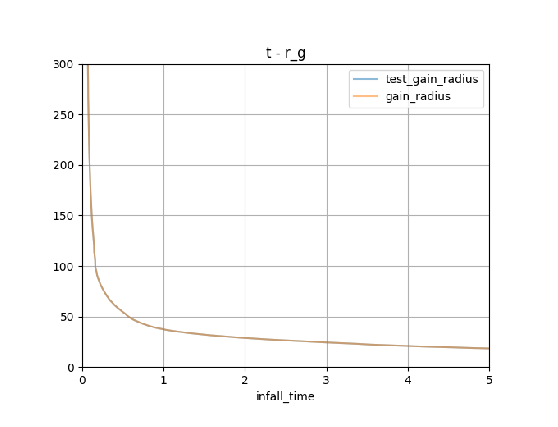
\includegraphics[width=130mm]{./img/s12M_r_g_t.eps}}
  \end{center}
  \caption{m\"{u}llerのデータとの比較($r_g$)}
  \label{fig:compare_1}
\end{figure}
\begin{figure}[htbp]
  \begin{center}
    \fbox{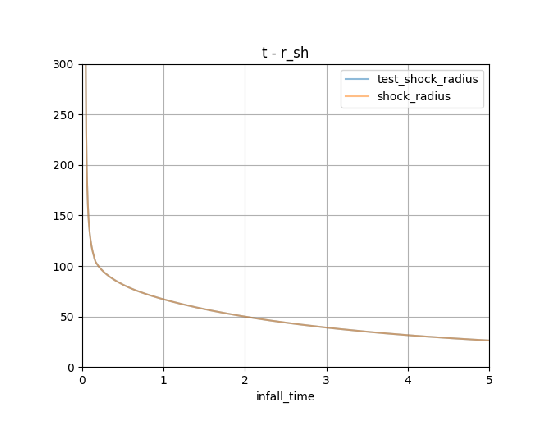
\includegraphics[width=130mm]{./img/s12M_r_sh_t.eps}}
  \end{center}
  \caption{m\"{u}llerのデータとの比較($r_{sh}$)}
  \label{fig:compare_2}
\end{figure}
\begin{figure}[htbp]
  \begin{center}
    \fbox{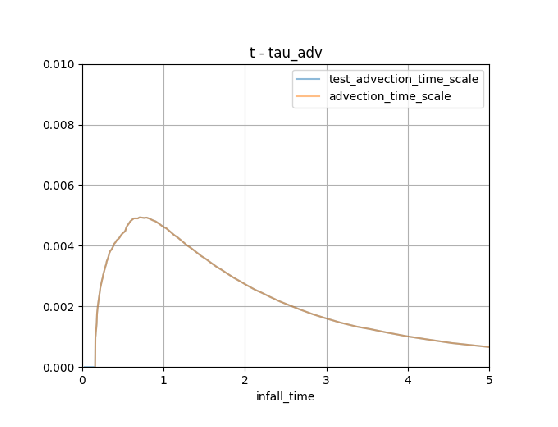
\includegraphics[width=130mm]{./img/s12M_tau_adv_t.eps}}
  \end{center}
  \caption{m\"{u}llerのデータとの比較($\tau_{adv}$)}
  \label{fig:compare_3}
\end{figure}
\begin{figure}[htbp]
  \begin{center}
    \fbox{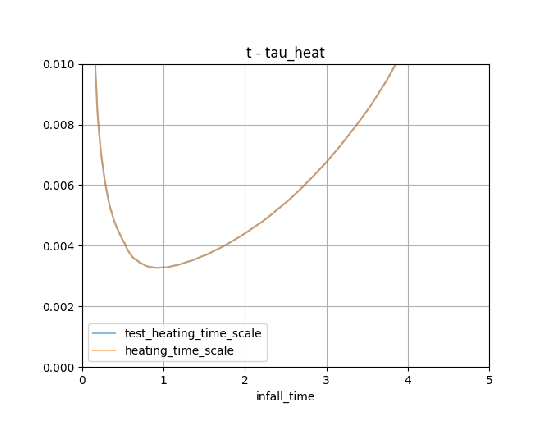
\includegraphics[width=130mm]{./img/s12M_tau_heat_t.eps}}
  \end{center}
  \caption{m\"{u}llerのデータとの比較($\tau_{heat}$)}
  \label{fig:compare_4}
\end{figure}
\begin{figure}[htbp]
  \begin{center}
    \fbox{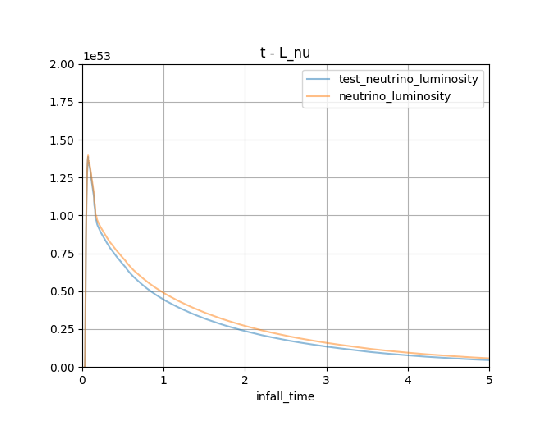
\includegraphics[width=130mm]{./img/s12M_L_nu_t.eps}}
  \end{center}
  \caption{m\"{u}llerのデータとの比較($L_{\nu}$)}
  \label{fig:compare_5}
\end{figure}
\begin{figure}[htbp]
  \begin{center}
    \fbox{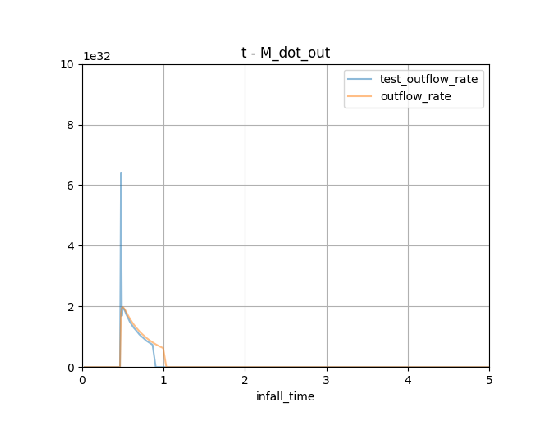
\includegraphics[width=130mm]{./img/s12M_M_dot_out_t.eps}}
  \end{center}
  \caption{m\"{u}llerのデータとの比較($\dot{M}_{out}$)}
  \label{fig:compare_6}
\end{figure}
\begin{figure}[htbp]
  \begin{center}
    \fbox{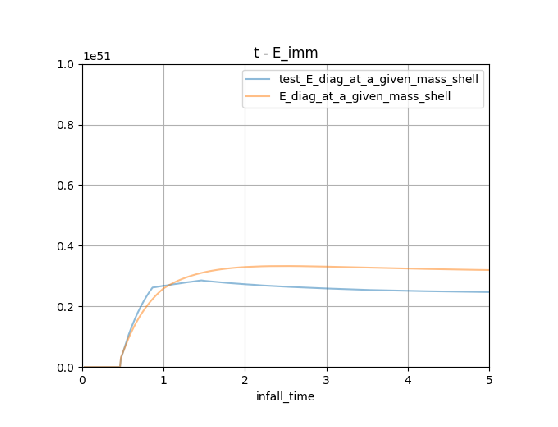
\includegraphics[width=130mm]{./img/s12M_E_imm_t.eps}}
  \end{center}
  \caption{m\"{u}llerのデータとの比較($E_{imm}$)}
  \label{fig:compare_7}
\end{figure}
\begin{figure}[htbp]
  \begin{center}
    \fbox{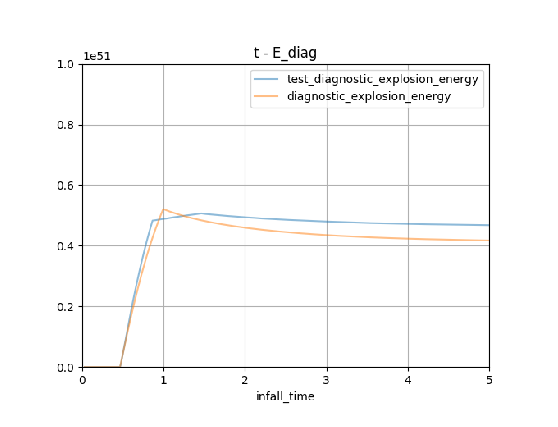
\includegraphics[width=130mm]{./img/s12M_E_diag_t.eps}}
  \end{center}
  \caption{m\"{u}llerのデータとの比較($E_{diag}$)}
  \label{fig:compare_8}
\end{figure}

\newpage

図\ref{fig:compare_1}$\sim$図\ref{fig:compare_4}までは完全に一致している.図\ref{fig:compare_5}$\sim$図\ref{fig:compare_8}では不一致の部分が目立つようになっていた.爆発段階での計算が少しずれていることが分かる.しかし,m\"{u}llerのデータの正確性が問われる状態なので大体の形が合っているということで計算の信ぴょう性は担保できたと判断した.

\section{計算例}

1つ例をあげて,$15M\sun$での計算結果の様子を紹介する.

このケースは爆発段階(Phase1)までは行くが,Phase2にはいかずにBHになる例である.

\begin{figure}[htbp]
  \begin{center}
    \fbox{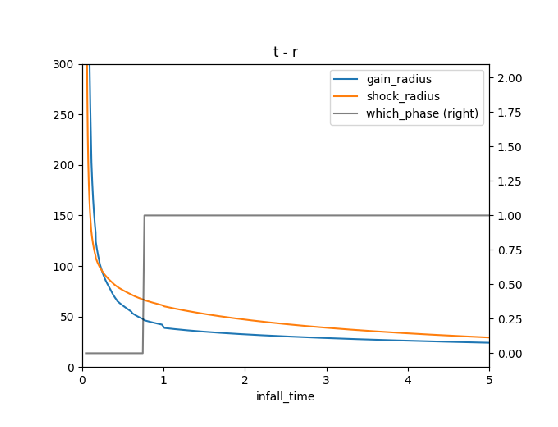
\includegraphics[width=130mm]{./img/woosley_s15.0_r_t.eps}}
  \end{center}
  \caption{ゲイン半径と衝撃波半径(woosly15.0M)}
  \label{fig:example_r_t}
\end{figure}

\begin{figure}[htbp]
  \begin{center}
    \fbox{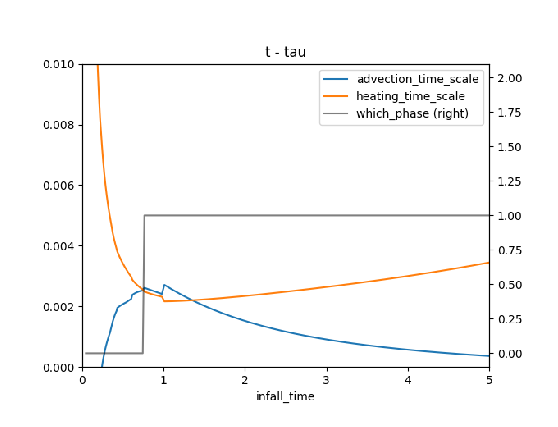
\includegraphics[width=130mm]{./img/woosley_s15.0_tau_t.eps}}
  \end{center}
  \caption{衝撃波復活の条件(woosly15.0M)}
  \label{fig:example_tau_t}
\end{figure}


\begin{figure}[htbp]
  \begin{center}
    \fbox{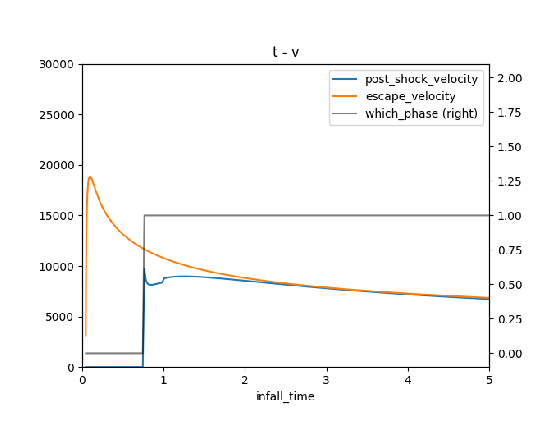
\includegraphics[width=130mm]{./img/woosley_s15.0_v_t.eps}}
  \end{center}
  \caption{Phase2へ移行できるか(woosly15.0M)}
  \label{fig:example_v_t}
\end{figure}

\begin{figure}[htbp]
  \begin{center}
    \fbox{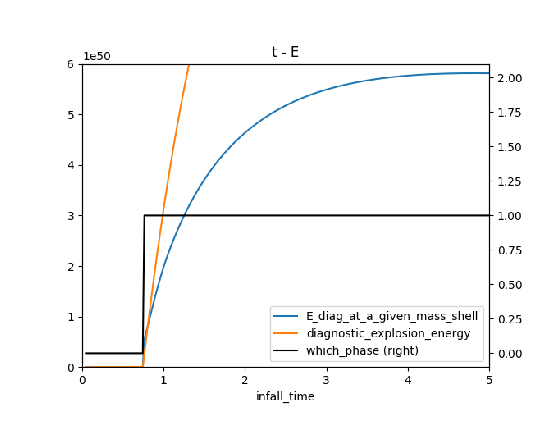
\includegraphics[width=130mm]{./img/woosley_s15.0_E_t.eps}}
  \end{center}
  \caption{爆発のエネルギー(woosly15.0M)}
  \label{fig:example_E_t}
\end{figure}

\newpage

\section{爆発結果}

全てのデータで爆発までの計算を行い.最終的な爆発のエネルギーと中性子星の質量を求めた.まずは,全体の中でどれくらいの星が爆発しているのかを見てみた.すると図\ref{fig:result_3}をみると分かるように,$25M\sun$から爆発しないという結果になった.$25M\sun$までに軸を拡大してみてみると,図\ref{fig:result_1}のようになる.右上のm\"{u}llerの論文でのグラフと比べると大きくズレがあることが分かる.


\begin{figure}[htbp]
  \begin{center}
    \fbox{\includegraphics[width=130mm]{./img/result_3.eps}}
  \end{center}
  \caption{爆発のエネルギー}
  \label{fig:result_3}
\end{figure}

\begin{figure}[htbp]
  \begin{center}
    \fbox{\includegraphics[width=130mm]{./img/result_1.eps}}
  \end{center}
  \caption{爆発のエネルギー(拡大)}
  \label{fig:result_1}
\end{figure}

\newpage
また,中性子星の質量についてもBHにならずに爆発を起こした部分なので$25M\sun$までに軸を拡大してみてみると,図\ref{fig:result_2}のようになる.これも右上のm\"{u}llerの論文上のグラフとは大きくずれていた.

\begin{figure}[htbp]
  \begin{center}
    \fbox{\includegraphics[width=130mm]{./img/result_2.eps}}
  \end{center}
  \caption{中性子星の質量(拡大)}
  \label{fig:result_2}
\end{figure}

\chapter{結論}
\label{chap:conclusion}

MESAを使って大量の親星を計算し,そのデータを元に爆発判定のプログラムを組むことができた.MESAで行う星の進化計算で星の進化についての理解を深めることができたの加え,メモリを気にしたコードの実行,並列処理の実装,bashコードによる作業の自動化等の学びを得ることができた.また,爆発判定を行うプログラムを作ることでニュートリノ加熱による衝撃波復活の流れを学ぶことができた.データとしては有効なものが取れたとは思えないが,他のパラメーターを用いて判定することもできるので発展として色々なパラメータを用いて様々な角度から比較したい.


\begin{acknowledgment}

本論文を作成するにあたり,1年間ゼミで指導していただいた鈴木教授,ならびにMESAの相談からちょっとした議論まで相談したときに真摯に相手にしていていただいたM2の大野木先輩に心から感謝を申し上げます.
  
\end{acknowledgment}
  
\begin{bib}[100]

  \bibitem{muller}
    M\"{u}ller,B., Heger,A., Liptai,D., \& Cameron,J.B.:
    \newblock A simple approach to the supernova progenitor-explosion connection,
    \newblock MNRAS, 2016
  
  \bibitem{woosly}
    wooslyの親星データ:
    \newblock https://2sn.org/stellarevolution/data.shtml

  \bibitem{mesa}
    mesaのドキュメント:
    \newblock http://mesa.sourceforge.net/

\end{bib}

\appendix

\end{document}
